\documentclass{standalone}
\usepackage{tikz}
\usetikzlibrary{patterns, angles}
\usepackage{circuitikz}

\begin{document}
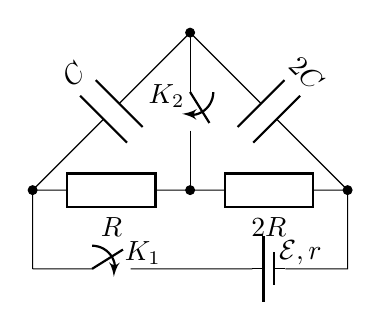
\begin{tikzpicture}[european]
	\draw (0,0) to [switch] (2,0) to [battery1] (4, 0) to [short, -*] (4,1) to [R=$2R$, -*] (2,1) to [R=$R$, -*] (0,1) -- (0,0);
	\draw (0,1) to [capacitor=$C$, -*] (2,3) to [capacitor=$2C$] (4,1);
	\draw (2, 3) to [switch] (2,1);
	\node at (3.4,0.2) {$\mathcal{E}, r$};
	\node at (1.4,0.2) {$K_1$};
	\node at (1.7,2.2) {$K_2$};
\end{tikzpicture}
\end{document}